%-----------------------------------------------------------------------------%
\chapter{\babEmpat}
%-----------------------------------------------------------------------------%
Pada bagian ini dijelaskan mengenai data hasil penelitian dan analisis data yang dilakukan oleh penulis. Hasil penelitian meliputi data demografi responden dan hasil pengolahan data yang diperoleh dari survei yang telah dilaksanakan pada masing-masing variabel pengukuran, analisis teori serta pengolahan rekomendasi responden pada penelitian.
%-----------------------------------------------------------------------------%
\section{Demografi Responden}
Pada penelitian ini responden adalah target pengguna dari \f{website} Direktorat Jenderal Pajak (DJP). Responden berjumlah 36 orang yang merupakan orang yang bekerja di bidang pajak serta mahasiswa dengan jurusan administrasi perpajakan(fiskal). Berikut merupakan grafik demografi dari responden penelitian.
\begin{figure}
	\centering
	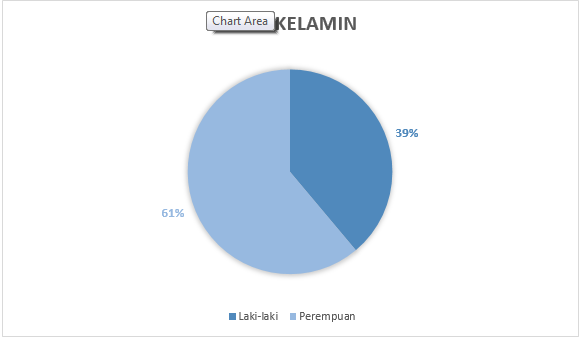
\includegraphics[width=0.9\textwidth,height=0.52\textwidth]
	{pics/jenisKelamin.PNG}
	\caption{Persentase jenis kelamin responden}
	\label{fig:jeniskelamin}
\end{figure}
\noindent
Gambar \ref{fig:jeniskelamin} menampilkan persentase data berdasarkan jenis kelamin responden. Diketahui dari gambar tersebut terdapat 14 orang laki-laki (39\%) dan 22 orang perempuan (61\%) yang menjadi responden. Gambar \ref{fig:kerja} merepresentasikan profesi yang dimiliki oleh responden berdasarkan jenisnya. Dari gambar dapat dilihat terdapat 19 orang (53\%) yang berprofesi sebagai konsultan pajak, 6 orang (17\%) pada bidang pajak lainnya dan 11 orang (30\%) mahasiswa dari jurusan administrasi perpajakan (fiskal).
\begin{figure}
	\centering
	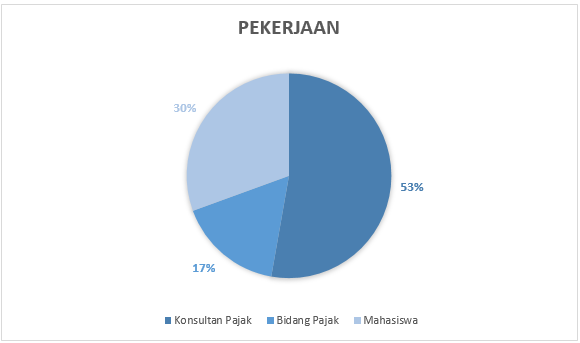
\includegraphics[width=0.9\textwidth,height=0.52\textwidth]
	{pics/pekerjaan.PNG}
	\caption{Persentase pekerjaan responden}
	\label{fig:kerja}
\end{figure}
\begin{figure}
	\centering
	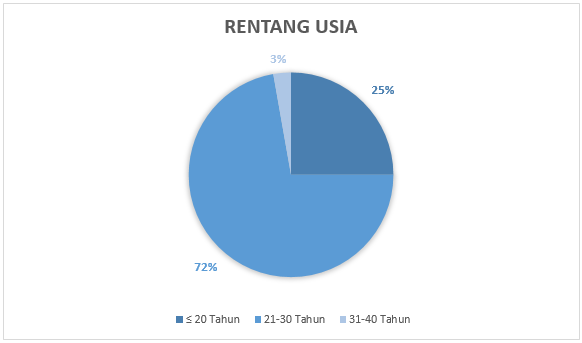
\includegraphics[width=0.9\textwidth,height=0.52\textwidth]
	{pics/rentangUsia.PNG}
	\caption{Persentase rentang usia responden}
	\label{fig:usia}
\end{figure}
\noindent
Gambar \ref{fig:usia} menggambarkan data persentase rentang usia responden penelitian. Diketahui dari gambar tersebut terdapat 1 orang (3\%) yang berusia pada rentang 31-40 tahun, 26 orang (72\%) yang berusia pada rentang 21-30 tahun serta 9 orang (25\%) responden yang berusia dibawah atau sama dengan 20 tahun.
\begin{figure}
	\centering
	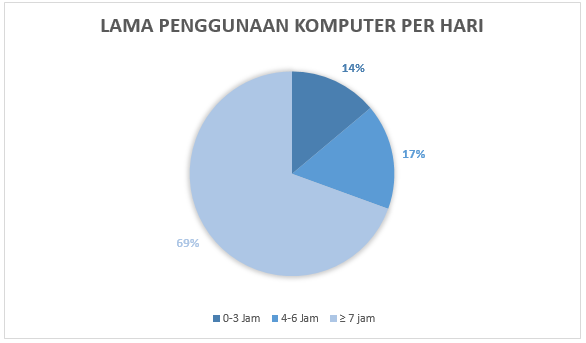
\includegraphics[width=0.9\textwidth,height=0.52\textwidth]
	{pics/lamakomputer.PNG}
	\caption{Persentase lama penggunaan komputer per hari responden}
	\label{fig:komp}
\end{figure}
\noindent
Gambar \ref{fig:komp} menunjukan persetase lama penggunaan komputer responden per hari. Sebanyak 5 orang (14\%) responden menggunakan komputer 0-3 Jam per hari, 6 orang (17\%) responden menggunakan komputer selama 4-6 jam per hari dan 25 oranng (69\%) responden menggunakan komputer selama lebih dari sama dengan 7 jam pada tiap harinya.
\begin{figure}
	\centering
	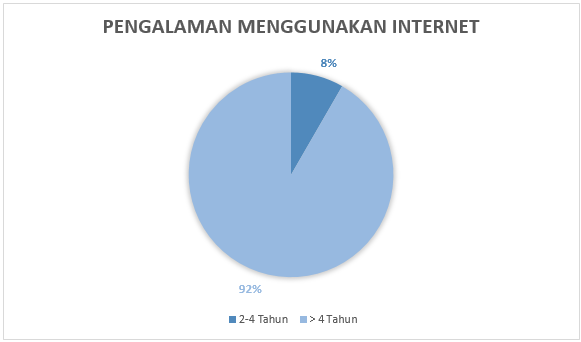
\includegraphics[width=0.9\textwidth,height=0.52\textwidth]
	{pics/pengalamanInternet.PNG}
	\caption{Persentase pengalaman responden menggunakan internet}
	\label{fig:lamainet}
\end{figure}
\noindent
Gambar \ref{fig:lamainet} menjelaskan mengenai persentasi pengalaman responden dalam menggunakan internet. Terdapat 3 orang (8\%) responden yang memiliki pengalaman menggunakan internet selama 2-4 tahun dn 33 orang (92\%) responden yang memiliki pengalaman menggunakan internet selama lebih dari 4 tahun.
\begin{figure}
	\centering
	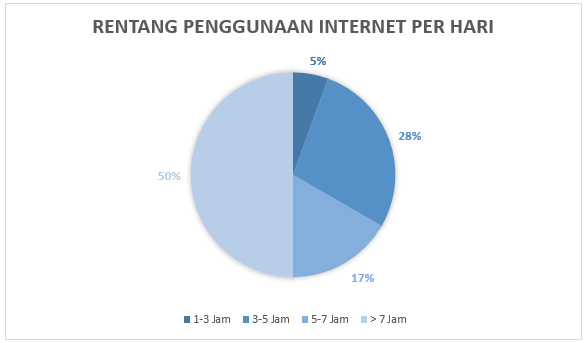
\includegraphics[width=0.9\textwidth,height=0.52\textwidth]
	{pics/pakeInternetperhari.PNG}
	\caption{Persentase rentang penggunaan internet per hari responden}
	\label{fig:maininet}
\end{figure}
\begin{figure}
	\centering
	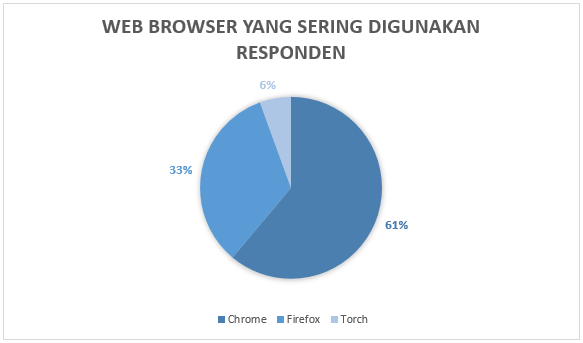
\includegraphics[width=0.9\textwidth,height=0.52\textwidth]
	{pics/webfavorit.PNG}
	\caption{Persentase \f{web browser} yang sering digunakan responden}
	\label{fig:browser}
\end{figure}
\noindent
Gambar \ref{fig:maininet} menjelaskan mengenai persentase rentang penggunaan internet per hari oleh responden. Sebanyak 2 orang (5\%) responden biasa menggunakan internet 1-3 jam per hari, 10 orang (28\%) responden menggunakan internet 3-5 jam per hari, 6 orang (17\%) responden menggunakan 5-7 jam per hari dan 18 orang (50\%) responden menggunakan internet lebih dari 7 jam. Gambar \ref{fig:browser} menunjukan mengenai persentase \f{web browser} yang sering digunakan oleh responden. Terdapat 22 orang (61\%) responden yang biasa menggunakan \f{web browser Google Chrome}, 12 orang (33\%) responden biasa menggunakan \f{web browser Mozilla Firefox} dan 2 orang (6\%) responden biasa menggunakan \f{web browser Torch}.
\begin{figure}
	\centering
	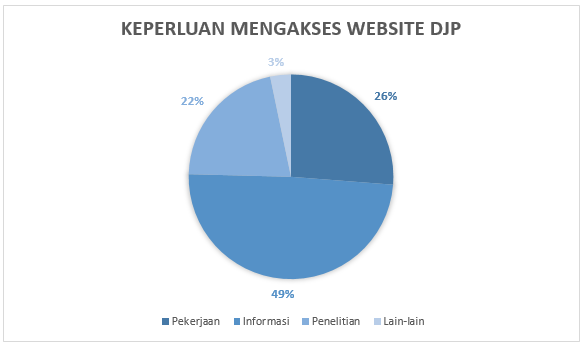
\includegraphics[width=0.9\textwidth,height=0.52\textwidth]
	{pics/keperluanAkses.PNG}
	\caption{Persentase keperluan akses \f{website} DJP Indonesia}
	\label{fig:akses}
\end{figure}
\noindent
Dari data penelitian diketahui bahwa semua responden pernah mengakses \f{website} Direktorat Jenderal Pajak (DJP) Indonesia. Gambar \ref{fig:akses} menjelaskan mengenai persentase keperluan responden mengakses \f{website} Direktorat Jenderal Pajak (DJP) Indonesia. Sebanyak 49\% responden menyatakan keperluan mereka mengakses \f{website} DJP untuk informasi, 26\% responden menyatakan keperluan akses untuk pekerjaan, 22\% responden menyatakan untuk penelitian dan 3\% responden menyatakan keperluan akses \f{website} DJP untuk hal lain-lain.
%-----------------------------------------------------------------------------%
\section{Uji Validitas dan Reliabilitas}
Pada bagian ini dijelaskan mengenai uji validitas dan reliabilitas dari instrumen kuesioner penelitian yang digunakan oleh penulis.
%-----------------------------------------------------------------------------%
\subsection{Uji Validitas}
Uji validitas dilakukan oleh penulis untuk menguji apakah data instrumen penelitian yang digunakan valid atau tidak, instrumen dalam penelitian ini adalah kuesioner yang digunakan untuk pengumpulan data. Pengujian dilakukan menggunakan metode Cronbach's Alpha, pengujian dilakukan dengan melakukan perbandingan nilai \f{corrected item-total correlation} terhadap taraf signifikansi 0.05 \citep{buku.riduwan}. Berikut merupakan kriteria dari pengujian ini.
\begin{itemize}
	\item Bernilai valid jika nilai dari \f{corrected item-total correlation value} (r hitung)  $\geq$ r tabel \f{product moment} dengan derajat kebebasan N-1.
	\item Bernilai tidak valid jika nilai dari \f{corrected item-total correlation value} (r hitung)  $\leq$ r tabel \f{product moment} dengan derajat kebebasan N-1.
\end{itemize}
\begin{table}
	\centering
	\caption{Hasil uji validitas terhadap komponen \f{usability heuristic}.}
	\label{tab:ujivaliditasuh}
	\begin{tabular}{c}
		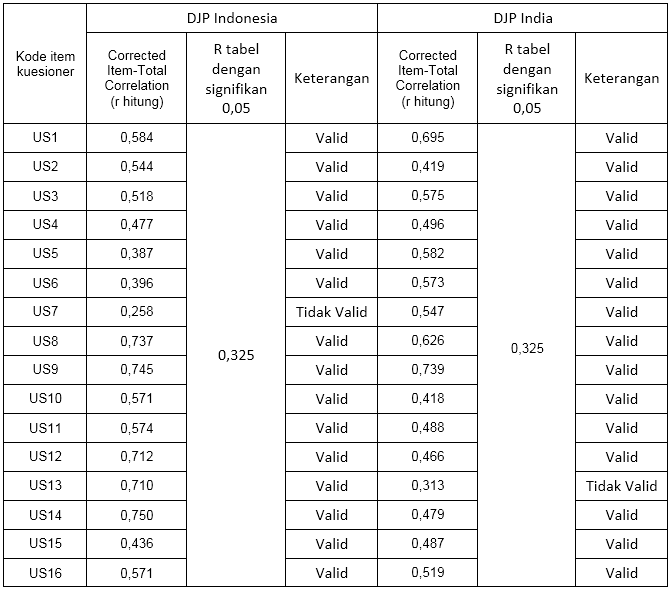
\includegraphics[width=\textwidth]
		{pics/validitasUsabilityHeuristic.PNG}
\end{tabular}
\end{table}
Tabel \ref{tab:ujivaliditasuh} menunjukan bahwa masing-masing data pertanyaan terdapat sebuah nilai yang tidak valid pada komponen \f{usability heuristic} bila dilihat hasil perbandingan r hitung dengan r tabel \f{product moment}. Hal ini disebabkan dari persebaran variatif data yang nilainya kurang signifikan.
\newline\\
Selanjutnya tabel \ref{tab:ujivaliditassat} menerangkan bahwa bahwa semua unit dalam komponen kepuasan pengguna memiliki data yang sudah valid. Nilai pada kolom r-hitung bila dibandingkan denga r-tabel bernilai lebih besar sehingga nilai data valid.
\begin{table}
	\centering
	\caption{Hasil uji validitas terhadap komponen kepuasan pengguna.}
	\label{tab:ujivaliditassat}
	\begin{tabular}{c}
		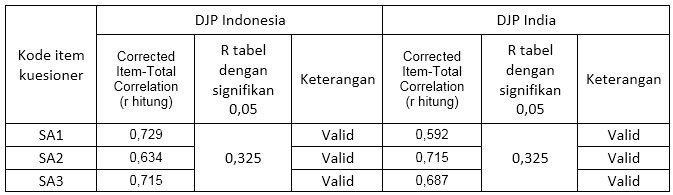
\includegraphics[width=\textwidth]
		{pics/validitasKepuasanPengguna.PNG}
	\end{tabular}
\end{table}
\noindent
Pada tabel \ref{tab:ujivaliditasgq} dapat dilihat nilai r-hitung dari data yang terdapat pada komponen \f{g-Quality} yang ternyata setelah dibandingkan dengan r-tabel terdapat dua buah data yang tidak valid baik di data pengujian DJP Indonesia maupun DJP India.
\begin{table}
	\centering
	\caption{Hasil uji validitas terhadap komponen \f{g-Quality}.}
	\label{tab:ujivaliditasgq}
	\begin{tabular}{c}
		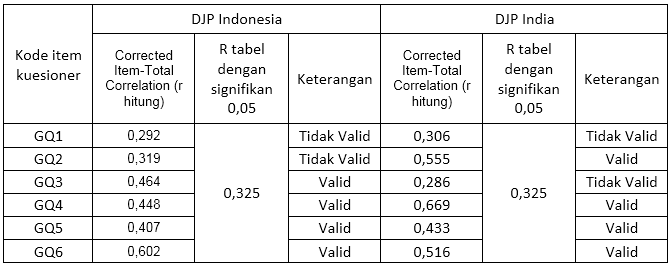
\includegraphics[width=\textwidth]
		{pics/validitasGQuality.PNG}
	\end{tabular}
\end{table}
%-----------------------------------------------------------------------------%
\subsection{Uji Realibilitas}
Uji reliabilitas digunakan untuk menguji instrumen kuesioner yang digunakan pada penelitian terpercaya atau reliabel \citep{article.raharjo}. Uji reliabilitas dilakukan untuk mengetahui tingkat kekonsistenan instrumen kuesioner yang digunakan dalam penelitian. \citet{buku.george} menyatakan bahwa belum ada standar yang mengenai nilai Cronbach's Alpha yang memenuhi nilai acceptable. \citet{buku.george} mambagi nilai dari alpha menjadi 5 bagian dalam tabel \ref{tab:cronalpha} untuk menentukan apakah konsistensi suatu instrumen dapat diterima atau tidak.
\begin{table}
	\centering
	\caption{Kategori Cronbach's Alpha}
	\label{tab:cronalpha}
	\begin{tabular}{|l|l|}
		\hline
		\multicolumn{1}{|c|}{\bf Cronbach's Alpha} & \multicolumn{1}{c|}{{\bf Internal Consistency}} \\ \hline
		a $\geq$ 0.9 & Excellent (High-Stakes testing) \\ \hline
		0.7 $\leq$ a < 0.8 & Good (Low-Stakes testing) \\ \hline
		0.6 $\leq$ a < 0.7 & Acceptable  \\ \hline
		0.5 $\leq$ a < 0.6 & Poor   \\ \hline
		a < 0.5           & Unacceptable  \\ \hline 
	\end{tabular}
		\begin{center}
			{\small Sumber tabel: \citep{buku.george}}
		\end{center}
\end{table}
Tabel \ref{tab:hasilconalp} berikut menunjukan hasil dari uji realibilitas instrumen kuesioner yang digunakan dalam penelitian. Terlihat bahwa komponen pada tiap kuesioner bernilai valid.
\begin{table}
	\centering
	\caption{Hasil penghitungan Cronbach's Alpha terhadap instrumen}
	\label{tab:hasilconalp}
	\begin{tabular}{|l|l|l|l|}
		\cline{2-4}
		\multicolumn{1}{c|}{} &
		\multicolumn{1}{l|}{\bf DJP Indonesia} &
		\multicolumn{1}{l|}{\bf DJP India} &
		\multicolumn{1}{l|}{{\bf Keterangan}} \\ \hline
		\f{Usability Heuristic} & 0,894
		 & 0,879 & Valid \\ \hline
		\f{Satisfaction} & 0,828
		& 0,812 & Valid \\ \hline
		\f{g-Quality} & 0,687
		 & 0,712 & Valid \\ \hline
	\end{tabular}
\end{table}
%-----------------------------------------------------------------------------%
\section{Analisis Data}
Pada bagian ini dijelaskan hasil penghitungan analisis data yang didapat dari instrumen dengan menggunakan aplikasi perangkat lunak SPSS 22. Analisis dilakukan dengan metode \f{paired samples T-test} bila data terdistribusi secara normal, namun jika data tidak terdistribusi secara normal maka digunakan metode \f{Wilcoxon Signed-Rank Test} untuk melihat nilai signifikansi hasil perbandingan.
%-----------------------------------------------------------------------------%
\subsection{\f{Usability Heuristic}}
Pada bagian ini tabel \ref{tab:descuh} menjelaskan bahwa nilai \f{mean} komponen \f{usability heuristic} pada \f{website} DJP India lebih besar dibandingkan dengan \f{website} DJP Indonesia. \f{Website} DJP Indonesia memiliki nilai \f{mean} 4,39409 sedangkan \f{website} DJP India memiliki nilai \f{mean} sebesar 5,42187. Selain nilai \f{mean}, tabel \ref{tab:descuh} juga menunjukan nilai \f{skewness} dan \f{kurtosis} dari masing-masing \f{website} pada komponen \f{usability heuristic}. Maka dapat diketahui nilai dari rasio \f{skewness} dan \f{kurtosis} pada kedua \f{website} tersebut. Nilai rasio \f{skewness} pada \f{website} DJP Indonesia adalah sebesar -0,182/0,393 = -0,4631 dan rasio \f{kurtosis}-nya adalah -0,35/0,768 = -1,0872, sedangkan pada \f{website} DJP India nilai rasio skewnes adalah -0,538/0,393 = -1,3689 dan nilai rasio \f{kurtosis}nya adalah 0,812/0,768 = 1,0572. Telah diketahui bahwa keempat nilai tersebut berada pada rentang -2 dan 2, sehingga dapat disimpulkan bahwa data terdistribusi secara normal. 
\begin{table}
	\centering
	\caption{Hasil statistik deskriptif terhadap komponen \f{usability heuristic}.}
	\label{tab:descuh}
	\begin{tabular}{c}
		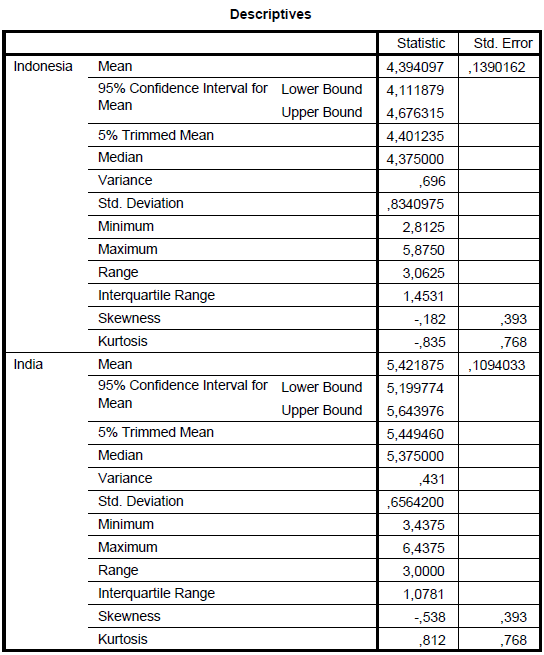
\includegraphics[width=\textwidth]
		{pics/ordinalDescUH.PNG}
	\end{tabular}
\end{table}
\noindent
Diketahui bahwa data terdistribusi secara normal, maka syarat \f{paired samples T-test} telah terpenuhi. Maka dilakukan penghitungan perbandingan nilai kedua \f{website} pada komponen \f{usability heuristic} sehingga diperoleh nilai seperti pada tabel \ref{tab:ttestuh}. Terlihat bahwa hasil \f{paired samples T-test} dalam tabel memiliki nilai signifikansi (Sig. (2-\f{tailed})) untuk komponen \f{usability heuristic} pada \f{website} DJP Indonesia dan India adalah 0,000 (\f{p} < 0,05), sehingga dapat disimpulkan bahwa \textbf{terdapat perbedaan yang signifikan pada komponen \f{usability heuristic} antara \f{website} DJP Indonesia dan DJP India}. Sehingga diketahui bahwa kualitas \f{usability} pada \f{website} DJP India terjaga dengan baik.
\begin{table}[h]
	\centering
	\caption{Hasil \f{paired samples T-test} terhadap komponen \f{usability heuristic}.}
	\label{tab:ttestuh}
	\begin{tabular}{c}
		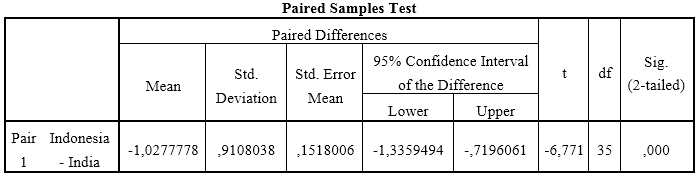
\includegraphics[width=\textwidth]
		{pics/ordinalT-testUH.PNG}
	\end{tabular}
\end{table}
Nilai \f{usability heuristic} pada \f{website} DJP India lebih tinggi dibandingkan dengan \f{website} DJP Indonesia, terlihat dari hasil \f{mean} pada tabel \ref{tab:rata2unituh} penilaian komponen \f{usability heuristic} \f{website} DJP India mendominasi dalam semua unit. Untuk lebih jelas perbandingan nilai \f{mean} setiap unit usablity heuristic, dapat dilihat histogram pada gambar \ref{fig:historata2uh}.
\begin{table}
	\centering
	\caption{Rata-rata nilai unit pada komponen \f{usability heuristic}}
	\label{tab:rata2unituh}
	\resizebox{\textwidth}{!}{%
		\begin{tabular}{ >{\centering\arraybackslash}m{1in} | >{\centering\arraybackslash}m{1in} | >{\centering\arraybackslash}m{1in} | >{\centering\arraybackslash}m{1in} |
				>{\centering\arraybackslash}m{1in} |
				>{\centering\arraybackslash}m{1in} |
				>{\centering\arraybackslash}m{1in} |
				>{\centering\arraybackslash}m{1in} |
				>{\centering\arraybackslash}m{1in} |
				>{\centering\arraybackslash}m{1in} |
				>{\centering\arraybackslash}m{1in} |
			}
			\cline{2-11}
			& UH1        & UH2        & UH3       & UH4       & UH5       & UH6       & UH7       & UH8       & UH9       & UH10 \\
			\hline
			\multicolumn{1}{|l|}{Indonesia} & 4,7777778 & 5,1388889 & 4,75     & 4,555556 & 3,916667 & 4,430556 & 4,87037  & 3,625    & 3,166667 & 4,2222222 \\
			\hline
			\multicolumn{1}{|l|}{India}     & 5,7222222 & 5,5555556 & 4,805556 & 5,361111 & 5,444444 & 5,375    & 5,425926 & 5,555556 & 5,305556 & 5,4166667 \\
			\hline
		\end{tabular}
	}
\end{table}

\begin{figure}
	\centering
	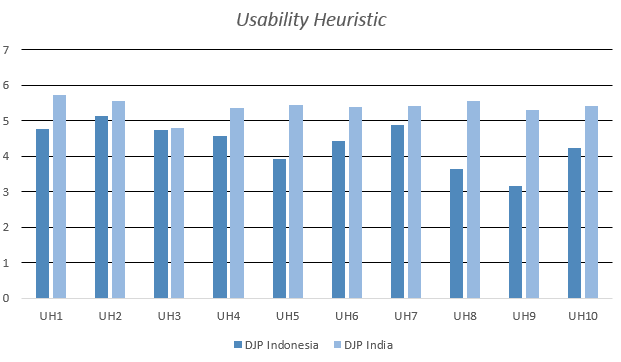
\includegraphics[width=\textwidth]
	{pics/historata2uh.PNG}
	\caption{Histogram \f{mean} unit pada komponen \f{usability heuristic}}
	\label{fig:historata2uh}
\end{figure}
\noindent
Keterangan tabel \ref{tab:rata2unituh} dan gambar \ref{fig:historata2uh}: \\
DJP Indonesia = \f{Website} Direktorat Jenderal Pajak Indonesia
DJP India = \f{Website} Direktorat Jenderal Pajak India
UH1 = \f{Visibility of system status} \\
UH2 = \f{Match between system and real world} \\
UH3 = \f{User control} \\
UH4 = \f{Consistency and standards} \\
UH5 = \f{Error prevention} \\
UH6 = \f{Recognition rather than recall} \\
UH7 = \f{Flexibility and efficiency of use} \\
UH8 = \f{Aesthetic and minimalist design} \\
UH9 = \f{Help user recognize, diagnose and recover from error} \\
UH10 = \f{Help and documentation}
%-----------------------------------------------------------------------------%
\subsection{Kepuasan Pengguna}
Tabel \ref{tab:descsat} menjelaskan bahwa nilai \f{mean} untuk komponen kepuasan pengguna \f{website} DJP India lebih unggul dibanding \f{website} DJP Indonesia. Hal tersebut dapat dilihat dengan nilai \f{mean} \f{website} DJP India yang bernilai 5,3611, sedangkan \f{website} DJP Indonesia memiliki nilai sebesar 4,6111. Selain nilai \f{mean}, dapat diketahui juga dari tabel \ref{tab:descsat} bahwa nilai rasio \f{skewness} untuk \f{website} DJP India adalah 0,070/0,393 = 0,17811 dan rasio \f{kurtosis}-nya -0,664/0,768 = 0,86458. Sedangkan untuk \f{website} DJP Indonesia diketahui bahwa rasio \f{skewness} sebesar -0,365/0,393 = -0,92875 dan rasio \f{kurtosis}-nya 0,309/0,768 = 0,40234. Dengan demikian diketahui bahwa nilai rasio \f{skewness} dan rasio \f{kurtosis} pada masing-masing komponen tingkat kepuasan pengguna terdistribusi secara normal karena terdapat pada rentang -2 dan 2. 
\begin{table}
	\centering
	\caption{Hasil statistik deskriptif terhadap komponen kepuasan pengguna}
	\label{tab:descsat}
	\begin{tabular}{c}
		\includegraphics[width=\textwidth]
		{pics/ordinaldescSAT.PNG}
	\end{tabular}
\end{table}
\noindent
Tabel \ref{tab:ttestsat} menunjukkan bahwa hasil analisa dengan metode \f{paired samples T-test} menunjukan bahwa komponen kepuasan pengguna memiliki nilai yang cukup signifikan dengan nilai signifikansi sebesar 0,003 (\f{p} < 0,05). Ini menunjukkan bahwa komponen tingkat kepuasan pengguna saat menggunakan \f{website} DJP Indonesia dan India \textbf{memiliki perbedaan yang signifikan}. Dari hasil tersebut diketahui bahwa kualitas \f{usability} dari DJP Indonesia kurang terjaga, hal tersebut dapat dilihat dari perbandingan \f{mean} tingkat kepuasan pengguna.
\begin{table}
	\centering
	\caption{Hasil \f{paired samples T-test} terhadap komponen kepuasan pengguna}
	\label{tab:ttestsat}
	\begin{tabular}{c}
		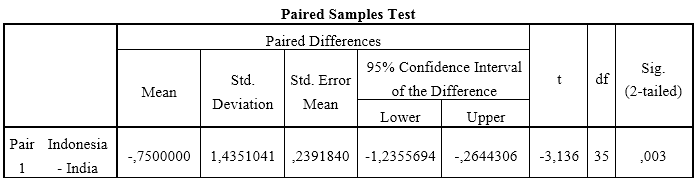
\includegraphics[width=\textwidth]
		{pics/ordinalT-testSAT.PNG}
	\end{tabular}
\end{table}
\noindent
%-----------------------------------------------------------------------------%
\subsection{Komponen \f{g-Quality}}
Pada tabel \ref{tab:descgq} dijelaskan bahwa nilai \f{mean} komponen \f{g-quality} pada \f{website} DJP India lebih besar dibandingkan dengan \f{website} DJP Indonesia. \f{Website} DJP Indonesia memiliki nilai \f{mean} 4,1111 sedangkan \f{website} DJP India memiliki nilai \f{mean} sebesar 5,2870. Selain nilai \f{mean}, tabel \ref{tab:descgq} juga menunjukan nilai \f{skewness} dan \f{kurtosis} dari masing-masing \f{website} pada komponen \f{g-quality}. Maka diketahui nilai rasio \f{skewness} dan \f{kurtosis} pada kedua \f{website} tersebut. Nilai rasio \f{skewness} pada \f{website} DJP Indonesia adalah sebesar -0,554/0,393 = -1,4096 dan rasio \f{kurtosis} sebesar -0,747/0,768 = -0,9726, pada \f{website} DJP India nilai rasio skewnes adalah -0,638/0,393 = -1,6324 dan nilai rasio \f{kurtosis}nya adalah 1,361/0,768 = 1,7721. Jelas bahwa keempat nilai tersebut berada pada rentang -2 dan 2, sehingga dapat disimpulkan bahwa data terdistribusi secara normal. 
\begin{table}
	\centering
	\caption{Hasil statistik deskriptif terhadap komponen \f{g-Quality}}
	\label{tab:descgq}
	\begin{tabular}{c}
		\includegraphics[width=\textwidth]
		{pics/ordinaldescGQ.PNG}
	\end{tabular}
\end{table}
\noindent
Setelah diketahui data terdistribusi secara normal, maka analisa \f{paired samples T-test} dilakukan untuk penghitungan perbandingan nilai kedua \f{website} pada komponen \f{g-quality} sehingga diperoleh nilai seperti pada tabel \ref{tab:ttestgq}. Terlihat bahwa hasil \f{paired samples T-test} dalam tabel memiliki nilai signifikansi (Sig. (2-\f{tailed})) untuk komponen \f{g-quality} pada \f{website} DJP Indonesia dan India adalah 0,000 (\f{p} < 0,05), sehingga dapat disimpulkan bahwa \textbf{terdapat perbedaan yang signifikan pada komponen \f{g-quality} antara \f{website} DJP Indonesia dan DJP India}. Sehingga diketahui bahwa kualitas \f{usability} pada \f{website} DJP India terjaga baik.
\begin{table}
	\centering
	\caption{Hasil \f{paired samples T-test} terhadap komponen \f{g-quality}}
	\label{tab:ttestgq}
	\begin{tabular}{c}
		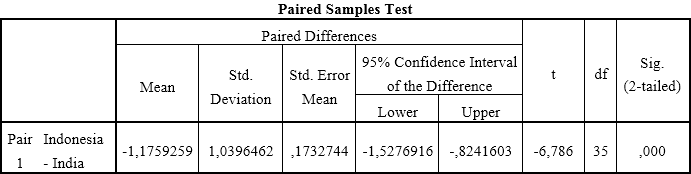
\includegraphics[width=\textwidth]
		{pics/ordinalT-testGQ.PNG}
	\end{tabular}
\end{table}
\noindent
Nilai \f{g-quality} pada \f{website} DJP India lebih tinggi dibandingkan dengan \f{website} DJP Indonesia, terlihat dari hasil \f{mean} pada tabel \ref{tab:rata2unitgq} penilaian komponen \f{g-quality} \f{website} DJP India mendominasi dalam semua unit. Untuk lebih jelas perbandingan nilai \f{mean} setiap unit usablity heuristic, dapat dilihat histogram pada gambar \ref{fig:historata2gq}.
\begin{table}
	\centering
	\caption{Rata-rata nilai unit pada komponen \f{g-quality}}
	\label{tab:rata2unitgq}
	\resizebox{\textwidth}{!}{%
		\begin{tabular}{ >{\centering\arraybackslash}m{1in} | >{\centering\arraybackslash}m{1in} | >{\centering\arraybackslash}m{1in} | >{\centering\arraybackslash}m{1in} |
				>{\centering\arraybackslash}m{1in} |
				>{\centering\arraybackslash}m{1in} |
				>{\centering\arraybackslash}m{1in} |
			}
			\cline{2-7}
			& GQ1        & GQ2        & GQ3       & GQ4       & GQ5       & GQ6  \\
			\hline
			\multicolumn{1}{|l|}{Indonesia} & 3,944444444 & 4,333333333 & 3,833333333 & 4,5 & 4 & 4,055555556 \\ \hline
			\multicolumn{1}{|l|}{India}     & 4,444444444 & 5,472222222 & 5,611111111 & 5,527777778 & 5,527777778 & 5,138888889 \\ \hline
		\end{tabular}
	}
\end{table}

\begin{figure}
	\centering
	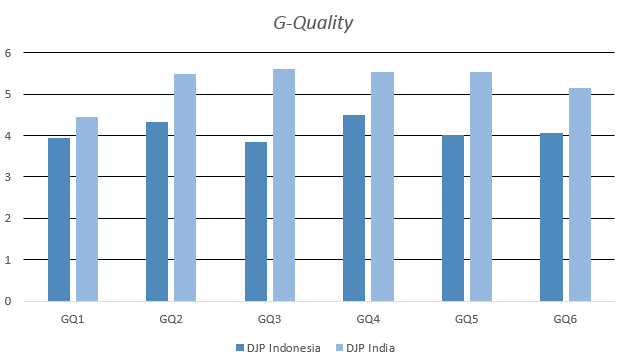
\includegraphics[width=\textwidth]
	{pics/historata2gq.PNG}
	\caption{Histogram \f{mean} unit pada komponen \f{g-quality}}
	\label{fig:historata2gq}
\end{figure}
\pagebreak

\noindent
Keterangan tabel \ref{tab:rata2unitgq} dan gambar \ref{fig:historata2gq}: \\
DJP Indonesia = \f{Website} Direktorat Jenderal Pajak Indonesia
DJP India = \f{Website} Direktorat Jenderal Pajak India
GQ1 = \f{Accessibility} \\
GQ2 = \f{Interoperability} \\
GQ3 = \f{Security and privacy} \\
GQ4 = \f{Information reliability} \\
GQ5 = \f{Service agility} \\
GQ6 = \f{Transparency} \\
%-----------------------------------------------------------------------------%
\subsection{Efisiensi}
Efisiensi dapat diukur dengan mengukur berapa banyak waktu yang digunakan oleh responden untuk menyelesaikan tugas yang diberikan, seperti yang telah dijelaskan sebelumnya pada subbab \ref{subsec:usability}. Diketahui dari tabel \ref{tab:descwaktu} bahwa \f{mean} lama waktu pengerjaan tugas pada \f{website} DJP Indonesia lebih besar dibandingkan dengan \f{website} DJP India. \f{Website} DJP Indonesia memiliki \f{mean} waktu selama 755,94 detik, sedangkan \f{website} DJP India memiliki \f{mean} waktu selama 670,13. Selain \f{mean} waktu pengerjaan tugas, tabel \ref{tab:descwaktu} juga menunjukan nilai \f{skewness} dan \f{kurtosis} dari masing-masing \f{website} pada lama waktu pengerjaan tugas. Maka diketahui nilai rasio \f{skewness} dan \f{kurtosis} pada kedua \f{website} tersebut. Nilai rasio \f{skewness} pada \f{website} DJP Indonesia adalah sebesar 0,601/0,393 = 1,529 dan rasio \f{kurtosis} sebesar -0,869/0,768 = -1,131, pada \f{website} DJP India nilai rasio skewnes adalah 0,424/0,393 = 1,078 dan nilai rasio \f{kurtosis}nya adalah -0,971/0,768 = -1,264. Jelas bahwa keempat nilai tersebut berada pada rentang -2 dan 2, sehingga dapat disimpulkan bahwa data terdistribusi secara normal. 
\begin{table}
	\centering
	\caption{Hasil statistik deskriptif terhadap lama waktu pengerjaan tugas}
	\label{tab:descwaktu}
	\begin{tabular}{c}
		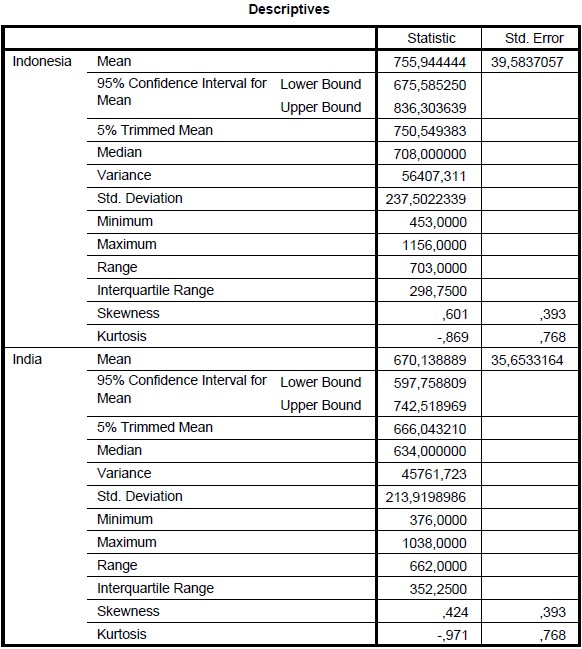
\includegraphics[width=\textwidth]
		{pics/waktudesc.PNG}
	\end{tabular}
\end{table}
\noindent
Setelah diketahui data terdistribusi secara normal, maka analisa \f{paired samples T-test} dilakukan untuk penghitungan perbandingan nilai kedua \f{website} pada lama waktu pengerjaan tugas sehingga diperoleh nilai seperti pada tabel \ref{tab:ttestwaktu}. Terlihat bahwa hasil \f{paired samples T-test} dalam tabel memiliki nilai signifikansi (Sig. (2-\f{tailed})) untuk lama waktu pengerjaan tugas pada \f{website} DJP Indonesia dan India adalah 0,000 (\f{p} < 0,05), sehingga dapat disimpulkan bahwa \textbf{terdapat perbedaan yang signifikan terhadap lama waktu pengerjaan tugas antara \f{website} DJP Indonesia dan DJP India}. Sehingga diketahui bahwa responden lebih banyak menghabiskan waktu pada \f{website} DJP Indonesia walau sesungguhnya \f{website} DJP India menggunakan bahasa yang bukan bahasa utama di negara Indonesia, selain itu \f{website} DJP Indonesia memuat banyak konten dalam satu halaman sehingga membuat bingung responden untuk mencari menu dan tugas yang dimaksud.
\begin{table}
	\centering
	\caption{Hasil \f{paired samples T-test} terhadap lama waktu pengerjaan tugas}
	\label{tab:ttestwaktu}
	\begin{tabular}{c}
		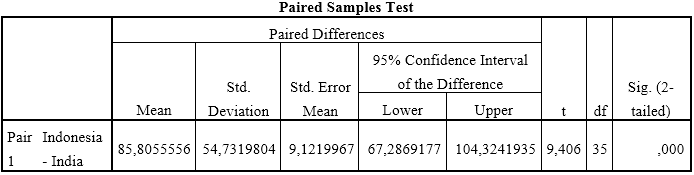
\includegraphics[width=\textwidth]
		{pics/waktuSelesaiT-test.PNG}
	\end{tabular}
\end{table}
%-----------------------------------------------------------------------------%
\subsection{Efektivitas}
Efektivitas dapat diukur dengan menghitung keberhasilan pengguna dalam mengerjakan tugas yang diberikan. Pada tabel \ref{tab:desctugasselesai} terlihat bahwa \f{mean} tugas yang berhasil dikerjakan pada \f{website} DJP India lebih banyak dibandingkan dengan \f{website} DJP Indonesia. \f{Website} DJP Indonesia memiliki \f{mean} tugas yang berhasil dikerjakan sebanyak 9,5833, sedangkan \f{website} DJP India memiliki \f{mean} tugas berhasil dikerjakan sebanyak 9,6944. Selain \f{mean} tugas yang berhasil dikerjakan, tabel \ref{tab:desctugasselesai} juga menunjukan nilai \f{skewness} dan \f{kurtosis} dari masing-masing \f{website} dalam tugas yang berhasil dikerjakan. Maka diketahui nilai rasio \f{skewness} dan \f{kurtosis} pada kedua \f{website} tersebut. Nilai rasio \f{skewness} pada \f{website} DJP Indonesia adalah sebesar -2,213/0,393 = -5,631 dan rasio \f{kurtosis} sebesar 3,823/0,768 = 4,977, pada \f{website} DJP India nilai rasio skewnes adalah -2,520/0,393 = -6,412 dan nilai rasio \f{kurtosis}nya adalah 6,123/0,768 = 8,024. Dari data sebelumnya terlihat bahwa keempat nilai tersebut tidak berada pada rentang -2 dan 2, sehingga dapat disimpulkan bahwa data tidak terdistribusi secara normal. Dikarenakan data yang tidak terdistribusi normal maka dilakukan transformasi dan pengujian ulang, namun data masih tetap tidak terdistribusi secara normal. Setelah mengetahui bahwa data tidak dapat ditransformasi maka digunakan penghitungan perbandingan non-parametrik menggunakan metode \f{Wilcoxon Signed Rank Test} sebagai pengganti \f{paired samples T-test}.
\begin{table}
	\centering
	\caption{Hasil statistik deskriptif terhadap tugas yang berhasil dikerjakan}
	\label{tab:desctugasselesai}
	\begin{tabular}{c}
		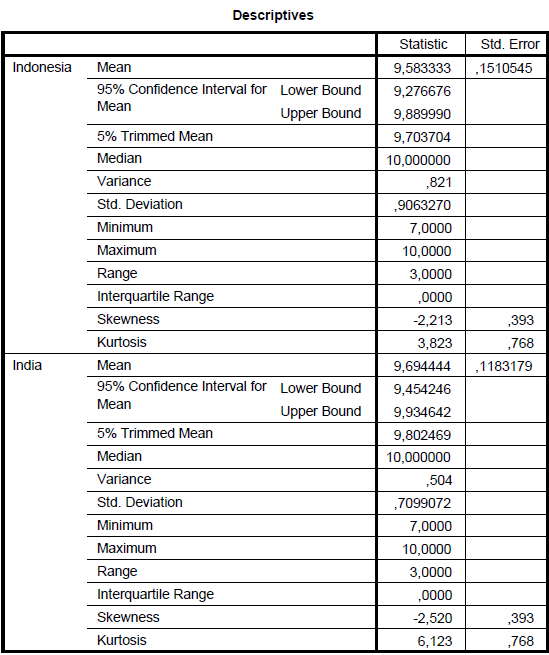
\includegraphics[width=\textwidth]
		{pics/tugasselesaidesc.PNG}
	\end{tabular}
\end{table}
Terlihat bahwa hasil \f{wilcoxon signed rank test} dalam tabel \ref{tab:hasiltugasselesai} memiliki nilai signifikansi (Sig. (2-\f{tailed})) untuk tugas yang berhasil dikerjakan pada \f{website} DJP Indonesia dan India adalah 0,285 (\f{p} > 0,05), sehingga dapat disimpulkan bahwa \textbf{tidak terdapat perbedaan yang signifikan antara jumlah tugas yang berhasil dikerjakan pada \f{website} DJP Indonesia dan DJP India}. Sehingga diketahui bahwa responden hampir sama banyaknya menyelesaikan tugas dalam pengujian \f{website} DJP Indonesia dengan DJP India.
\begin{table}
	\centering
	\caption{Rank \f{wilcoxon signed rank test} terhadap tugas yang berhasil dikerjakan}
	\label{tab:ranktugasselesai}
	\begin{tabular}{c}
		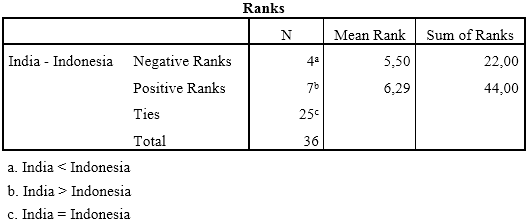
\includegraphics[width=\textwidth]
		{pics/rankSelesai.PNG}
	\end{tabular}
\end{table}
\begin{table}
	\centering
	\caption{Hasil \f{wilcoxon signed rank test} terhadap tugas yang berhasil dikerjakan}
	\label{tab:hasiltugasselesai}
	\begin{tabular}{c}
		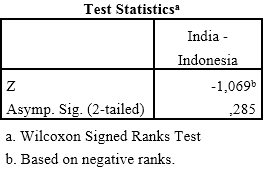
\includegraphics[width=0.5\textwidth]
		{pics/selesaiWilcoxon.PNG}
	\end{tabular}
\end{table}
%-----------------------------------------------------------------------------%
\subsection{Tingkat Kesalahan Pengguna}
Pengukuran tingkat kelasahan pengguna dilakukan dengan melakukan pencatatan terhadap pengerjaan tugas yang gagal dilakukan oleh pengguna pada pengujian \f{website} DJP Indonesia dengan India. Pada tabel \ref{tab:tugasgagaldesc} terlihat bahwa \f{mean} kesalahan yang dilakukan pengguna pada \f{website} DJP Indonesia lebih banyak dibandingkan dengan \f{website} DJP India. \f{Website} DJP Indonesia memiliki \f{mean} tugas yang gagal dikerjakan sebanyak 0,4166, sedangkan \f{website} DJP India memiliki \f{mean} tugas yang gagal dikerjakan sebanyak 0,0653. Selain \f{mean} tugas yang gagal dikerjakan, tabel \ref{tab:desctugasselesai} juga menunjukan nilai \f{skewness} dan \f{kurtosis} dari masing-masing \f{website} dalam tugas yang gagal dikerjakan. Maka diketahui nilai rasio \f{skewness} dan \f{kurtosis} pada kedua \f{website} tersebut. Nilai rasio \f{skewness} pada \f{website} DJP Indonesia adalah sebesar 2,213/0,393 = 5,631 dan rasio \f{kurtosis} sebesar 3,823/0,768 = 4,977, pada \f{website} DJP India nilai rasio skewnes adalah 2,520/0,393 = 6,412 dan nilai rasio \f{kurtosis}nya adalah 6,123/0,768 = 8,024. Dari data sebelumnya terlihat bahwa keempat nilai tersebut tidak berada pada rentang -2 dan 2, sehingga dapat disimpulkan bahwa data tidak terdistribusi secara normal. Dikarenakan data yang tidak terdistribusi normal maka dilakukan transformasi dan pengujian ulang, namun data masih tetap tidak terdistribusi secara normal. Setelah mengetahui bahwa data tidak dapat ditransformasi maka digunakan penghitungan perbandingan non-parametrik menggunakan metode \f{Wilcoxon Signed Rank Test} sebagai pengganti \f{paired samples T-test}.
\begin{table}
\centering
\caption{Hasil statistik deskriptif terhadap tugas yang gagal dikerjakan responden}
\label{tab:tugasgagaldesc}
\begin{tabular}{c}
	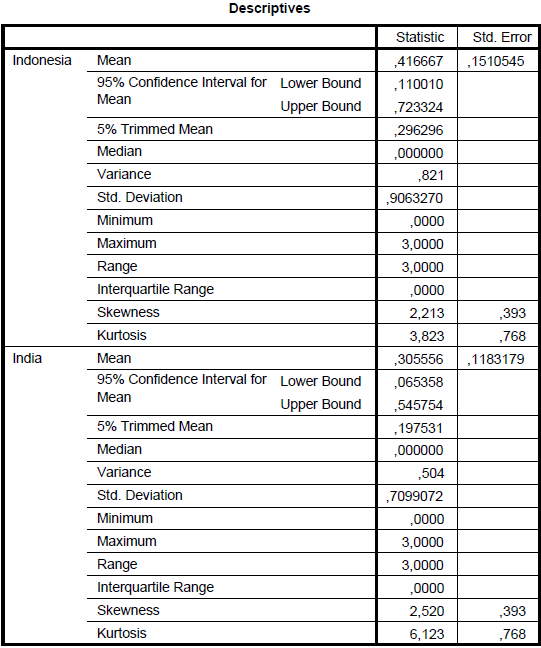
\includegraphics[width=\textwidth]
	{pics/tugasgagaldesc.PNG}
\end{tabular}
\end{table}
\noindent
Terlihat bahwa hasil \f{wilcoxon signed rank test} dalam tabel \ref{tab:hasiltugasgagal} memiliki nilai signifikansi (Sig. (2-\f{tailed})) untuk tugas yang gagal dikerjakan pada \f{website} DJP Indonesia dan India adalah 0,285 (\f{p} > 0,05), sehingga dapat disimpulkan bahwa \textbf{tidak terdapat perbedaan yang signifikan antara jumlah kesalahan yang dilakukan pengguna ketika menggunakan \f{website} DJP Indonesia dan DJP India}. Sehingga diketahui bahwa responden tidak terlalu banyak gagal menyelesaikan tugas dalam pengujian \f{website} DJP Indonesia dengan DJP India. Dari hasil observasi kesalahan yang terjadi dikarenakan penggunaan istilah yang tidak umum digunakan.
\begin{table}
	\centering
	\caption{Rank \f{wilcoxon signed rank test} terhadap tugas yang berhasil dikerjakan responden}
	\label{tab:ranktugasgagal}
	\begin{tabular}{c}
		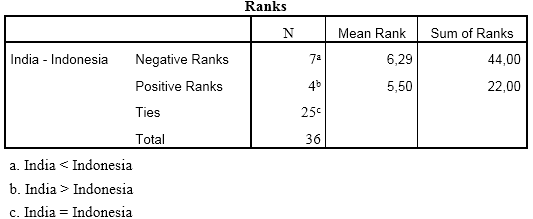
\includegraphics[width=\textwidth]
		{pics/rankGagal.PNG}
	\end{tabular}
\end{table}
\begin{table}
	\centering
	\caption{Hasil \f{wilcoxon signed rank test} terhadap tugas yang berhasil dikerjakan responden}
	\label{tab:hasiltugasgagal}
	\begin{tabular}{c}
		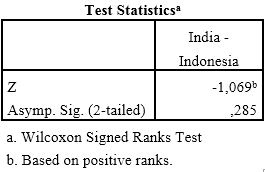
\includegraphics[width=0.5\textwidth]
		{pics/gagalWilcoxon.PNG}
	\end{tabular}
\end{table}
%-----------------------------------------------------------------------------%
\subsection{Preferensi Pengguna}
Dari hasil \f{open ended question} yang penulis berikan kepada responden terkait preferensi pengguna dalam menilai \f{website} DJP Indonesia dan India yang dibandingkan maka diperoleh hasil seperti pada gambar \ref{fig:preferensigraf}. Pada grafike gambar \ref{fig:preferensigraf} terlihat bahwa responden lebih cenderung memilih \f{website} DJP India.
Adapun beberapa alasan yang dikemukakan oleh responden memilih \f{website} DJP India sehingga menjadi dasar penilaian dengan penarikan kesimpulan sebagai berikut.
\begin{enumerate}
	\item Tampilan \f{website} DJP India lebih sederhana segingga mudah dimengerti dan digunakan, selain itu tampilan menarik karena banyak memberikan konten yang informatif.
	\item {Website} DJP India lebih mudah digunakan karena aksesnya cepat.
	\item Keamanan lebih baik pada \f{website} DJP India
	\item Penelusuran konten lebih mudah, sehingga pengguna merasa terbantu dan mudah mencari informasi yang dituju.
\end{enumerate}
Selain alasan memilih \f{website} DJP India diatas terdapat juga alasan terkait responden yang memilih \f{website} DJP Indonesia sebagai berikut.
\begin{enumerate}
	\item Sudah terbiasa menggunakan \f{website} DJP Indonesia.
	\item Fitur \f{e-filling} DJP Indonesia lebih bagus daripada DJP India.
	\item Konten yang dimiliki banyak.
\end{enumerate}

\begin{figure}
	\centering
	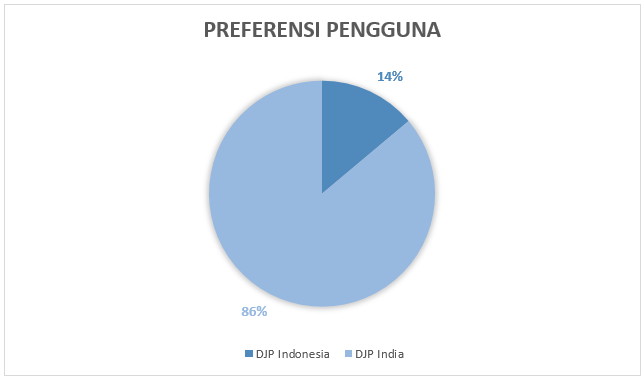
\includegraphics[width=\textwidth]
	{pics/preferensipengguna.PNG}
	\caption{Grafik preferensi pengguna terhadap \f{website} DJP Indonesia dan India}
	\label{fig:preferensigraf}
\end{figure}
\pagebreak
%-----------------------------------------------------------------------------%
\subsection{Analisa Perbandingan Teori}
Setelah mengetahui hasil analisa dari analisis perbandingan \f{usability testing} dan teori yang dikemukakan pada subbab \ref{subsec:gquality}. Maka dilakukan perbandingan penilaian \f{usability heuristic} dan \f{g-quality} berdasar lima kriteria evaluasi \f{e-government} sebagai berikut.
\begin{enumerate}
	\item \f{Cognitive Effort}\\
	Terlihat pada tabel \ref{tab:kriteriaegov} nilai yang dimiliki oleh \f{website} DJP Indonesia lebih rendah dari \f{website} DJP India. Penilaian cognitive effort didapat berdasarkan pencarian nilai dari penggolongan kriteria berdasarkan tabel \ref{tab:mappingegov}. Diketahui bahwa kedua \f{website} \f{e-government} memiliki nilai yang cukup berbeda, dimana \f{website} DJP Indonesia memiliki skor evaluasi sebesar \textbf{61,56} yang tergolong \textbf{cukup baik}, sedangkan \f{website} DJP India memiliki nilai sebesar \textbf{75,86} yang tergolong ke nilai yang \textbf{baik}. Sehingga dapat dijelaskan bahwa untuk mengakses \f{website} DJP Indonesia diperlukan usaha lebih untuk memahami terkait aspek kognitif dan menyesuaikan kebutuhan penggunaan sehingga pengguna harus mempelajari \f{website} agar dapat menggunakannya dengan lancar.
	\item \f{Tolerance}\\
	Pada tabel \ref{tab:kriteriaegov} terdapat perbedaan yang cukup signifikan pada kriteria toleransi untuk \f{website} DJP Indonesia dibanding India. Evaluasi terhadap kriteria ini menunjukkan bahwa \f{website} DJP Indonesia memiliki skor sebesar \textbf{58,36} yang digolongkan sebagai nilai yang \textbf{cukup}, sedangkan \f{website} DJP India mendapatkan skor \textbf{76,47} yang tergolong sebagai nilai \textbf{baik}. Hal ini menunjukkan bahwa \f{website} DJP Indonesia belum memberikan toleransi yang memuaskan terhadap pengguna yang dengan sabar menunggu, memahami dan melakukan aktivitas sesuai dengan respon dari \f{website}. 
	\item \f{Reach}\\
	Tabel \ref{tab:kriteriaegov} menunjukkan bahwa perbedaan nilai skor hasil evaluasi \f{usability} \f{e-government} antara \f{website} DJP Indonesia dan India memiliki jarak skor kriteria keterjangkauan yang paling dekat walau masih terpaut jauh dalam jumlah skor. Evaluasi terhadap kriteria ini menunjukkan bahwa \f{website} DJP Indonesia memiliki skor sebesar \textbf{63,39} yang tergolong \textbf{cukup baik}, sedangkan \f{website} DJP India memiliki skor sebesar \textbf{75,30} yang tergolong \textbf{baik}. Dengan demikian diketahui bahwa \f{website} DJP Indonesia masih memiliki kekurangan dalam keterjangkauan \f{website} kepada masyarakat.
	\item \f{Physical Effort}\\
	Pada tabel \ref{tab:kriteriaegov} diketahui bahwa \f{website} DJP Indonesia masih belum ungul dalam kriteria usaha fisik. Tabel \ref{tab:kriteriaegov} menunjukkan bahwa nilai skor hasil evaluasi \f{usability} \f{e-government} \f{website} DJP Indonesia memiliki skor sebesar \textbf{58,91} yang tergolong \textbf{cukup}, sedangkan \f{website} DJP India sebesar \textbf{77,16} yang tergolong \textbf{baik}. Hal ini menunjukkan bahwa \f{website} DJP Indonesia belum mudah untuk digunakan seperti pada hal penggunaan data yang kurang dimanfaatkan secara berulang-ulang.
	\item \f{Trust}\\
	Pada tabel \ref{tab:kriteriaegov} menunjukkan bahwa nilai skor pada kriteria kepercayaan dari \f{website} DJP Indonesia masih lebih rendah dibandingkan dengan \f{website} DJP India. \f{Website} DJP Indonesia memiliki skor sebesar \textbf{58,02} yang tergolong \textbf{cukup}, sedangkan \f{website} DJP India memiliki nilai \textbf{77,86} yang tergolong \textbf{baik}. Hal yang menyebabkan \f{website} DJP Indonesia memiliki nilai yang rendah pada kriteria ini karena masyarakat masih belum mempercayai \f{website} DJP Indonesia, fitur seperti keamanan akun masih dirasa kurang pada \f{website} DJP Indonesia sehingga menunjukkan bahwa \f{website} belum dapat dipercaya.
\end{enumerate}
Tabel \ref{tab:nilaiegov} menunjukkan nilai skor hasil evaluasi \f{usability website e-government} DJP Indonesia dan India per unit. Terlihat pada tabel untuk tiap unit komponen \f{website} DJP India mendominasi penilaian skor.
\begin{table}
	\centering
	\caption{Nilai dari evaluasi \f{usability e-government}}
	\label{tab:nilaiegov}
	\resizebox{\textwidth}{!}{%
		\begin{tabular}{|l|l|l|}
			\hline
			\multicolumn{1}{|c|}{\multirow{2}{*}{Komponen}} & \multicolumn{2}{c|}{Nilai Evaluasi (0$-$100\%)} \\ \cline{2-3} 
			& DJP Indonesia                                 & DJP India                                 \\ \hline
			\f{Visibility of system status} & 68,25 & 81,75 \\ \hline
			\f{Match between system and the real world} & 73,41 & 79,37 \\ \hline
			\f{User control and freedom} & 67,86 & 68,65 \\ \hline
			\f{Consistency and standards} & 65,08 & 76,59 \\ \hline
			\f{Error prevention} & 55,95 & 77,78 \\ \hline
			\f{Recognition rather than recall} & 63,29 & 76,79 \\ \hline
			\f{Flexibility and efficiency of use} & 69,58 & 77,51 \\ \hline
			\f{Aesthetics and minimalist design} & 51,79 & 79,37 \\ \hline
			\f{Help users recognize, diagnose, and recover from errors} & 45,24 & 75,79 \\ \hline
			\f{Help and documentation} & 60,32 & 77,38 \\ \hline
			\f{Accessibility} & 56,35 & 63,49 \\ \hline
			\f{Interoperability} & 61,90 & 78,17 \\ \hline
			\f{Security and privacy} & 54,76 & 80,16 \\ \hline
			\f{Information truth and precision} & 64,29 & 78,97 \\ \hline
			\f{Service Agility} & 57,14 & 78,97 \\ \hline
			\f{Transparency} & 57,94 & 73,41 \\ \hline
		\end{tabular}
	}
\end{table}
\begin{table}
	\centering
	\caption{Nilai evaluasi berdasarkan kriteria \f{e-government}}
	\label{tab:kriteriaegov}
	\begin{tabular}{|l|l|l|}
			\hline
			\multicolumn{1}{|c|}{\multirow{2}{*}{Kriteria}} & \multicolumn{2}{c|}{Nilai Evaluasi (0$-$100\%)} \\ \cline{2-3} 
			& DJP Indonesia                                 & DJP India                                   \\ \hline
			\f{Cognitive Effort}    & 61,56                                   & 75,86                                 \\ \hline
			\f{Tolerance}           & 58,36                                   & 76,47                                  \\ \hline
			\f{Reach}               & 63,39                                   & 75,30                                 \\ \hline
			\f{Physical Effort}     & 58,91                                   & 77,16                                 \\ \hline
			\f{Trust}               & 58,02                                   & 77,86                                 \\ \hline
		\end{tabular}
\end{table}
%-----------------------------------------------------------------------------%
\subsection{Rekomendasi Perbaikan}
Tabel \ref{tab:perbaikan} merupakan tabel rekomendasi perbaikan yang berhasil penulis himpun dari analisis data dan juga rekomendasi yang diberikan oleh responden. Tabel ini dijadikan dasar acuan untuk mengembangkan \f{high-fidelity prototyping}.
\begin{center}

\begin{longtable}{|p{0.5cm}|p{3.8cm}|p{3.8cm}|p{4.2cm}|}
	\caption{Rekomendasi perbaikan untuk \f{website} DJP Indonesia}
	\label{tab:perbaikan} \\
			\hline
			\textbf{No.} & \textbf{Rumusan Perbaikan} & \textbf{\f{Usability Heuristic}} & \textbf{Rekomendasi yang dirangkum dari Responden} \\ \hline \endhead
			1 & Perbaikan halaman \f{homepage} dari website DJP Indonesia agar lebih sederhana, dengan cara menggabungkan ulang menu dan desain ulang halaman. & \f{Aesthetic and minimalist design, match between system and the realworld, consystency and standards} dan \f{flexibility and efficiency of use.} & Perubahan tampilan yang lebih sederhana, rapih dan tata letak yang lebih baik.\\ \hline
			2 & Perbaikan halaman artikel dengan pengelompokkan tipe artikel dan informasi penyajian artikel. & \f{Consystency and standards, flexibility and efficiency of use, recognition rather than recall} dan \f{information truth and precision.} & Perbaiki dan perkaya konten sehingga lebih mudah mendapat informasi. \\ \hline
			3 & Perbaikan halaman \f{error} apabila pengguna melakukan kesalahan, serta halaman penanganannya. & \f{Error prevention, user control} dan \f{help user recognize, diagnose and recover from errors.} & Pemberitahuan terkait kesalahan seperti pencarian  \\ \hline
			4 & Perbaikan halaman download dengan pengelompokkan file yang lebih teratur dan rapih. & \f{Aesthetic and minimalist design, match between system and the realworld, consystency and standards, flexibility and efficiency of use} dan \f{recognition rather than recall.} & Halaman yang lebih rapih lagi.  \\ \hline
			5 & Perbaikan halaman aplikasi sebagai layanan penting yang ditawarkan kepada masyarakat. & \f{Aesthetic and minimalist design, match between system and the realworld, consystency and standards, flexibility and efficiency of use} dan \f{recognition rather than recall.} & Halaman aplikasi disatukan sehingga mudah diakses  \\ \hline
			6 & Perbaikan halaman login dari aplikasi \f{e-filling} untuk meningkatkan struktur keamanan. & \f{Security and privacy} & Perbaiki keamanan website sehingga merasa aman.  \\ \hline
			7 & Perbaikan halaman tutorial dan bentuk FAQ untuk mendukung pembelajaran terkait \f{website} kepada pengguna. & \f{Error prevention, help and documentation} dan \f{accessibility.} & Halaman FAQ dan tutorial yang lebih lengkap lagi. \\ \hline
			8 & Perbaikan halaman yang memberikan informasi terkait pengumuman sehingga memberikan informasi yang lebih akurat, terpercaya dan transparan & \f{Transparency} dan \f{information truth and precision.} & \f{Update} mengenai peraturan dan aturan yang dikelompokkan sehingga tersusun jelas. \\ \hline
			9   & Perbaikan halaman tautan antar \f{website e-government} sehingga aspek \f{interoperability} terpenuhi. & \f{Interoperability}. & Dapat akses informasi dengan website pemerintahan lain. \\ \hline
			10  & Perbaikan halaman layanan informasi sehingga aspek pelayanan lebih baik. & \f{Service agility}. & Informasi yang mudah didapat. \\ \hline
\end{longtable}
\end{center}

%-----------------------------------------------------------------------------%